\documentclass[12pt]{report}
\usepackage{amssymb}
\usepackage{amsmath}

\usepackage{multicol}
\usepackage{graphicx}
\usepackage{subfigure}
\usepackage{verbatim}


%\usepackage{adjustbox}

\usepackage[letterpaper,left=1cm,right=2cm, top=1.5cm,
bottom=1.5cm,head=0cm,foot=1cm]{geometry}

\parindent=0in


\newcommand{\m}{\mbox{ m }}
\newcommand{\kg}{\mbox{ kg }}
\newcommand{\s}{\mbox{ s }}
\newcommand{\ke}{\mbox{\small KE}}
\newcommand{\pe}{\mbox{\small PE}}


\newcommand{ \probDir}[1]{{ \bf\small #1 \mbox{  }}}

\newcommand{ \breakList}{\setcounter{saveenum}{\value{enumi}} \end{enumerate}}
\newcommand{ \contList}{\begin{enumerate} \setcounter{enumi}{\value{saveenum}}}

\newcounter{saveenum}

\def \wspace{5cm}

\graphicspath{ {./graphics/} }

%%%%%%%%%%%%%%%%%%%%%%%%%%%%%%%%%%%%%%%%%
\begin{document}

{\bf{Honors Physics} \hfill Notepage: Universal Gravitation \hfill {Mr. Kelley}} \\ \\
%%%%%%%%%%

\vspace{1cm}

\hfill \parbox{6cm}{\centering Matter attracts matter - we call this force gravity.} \hfill \raisebox{-2cm}{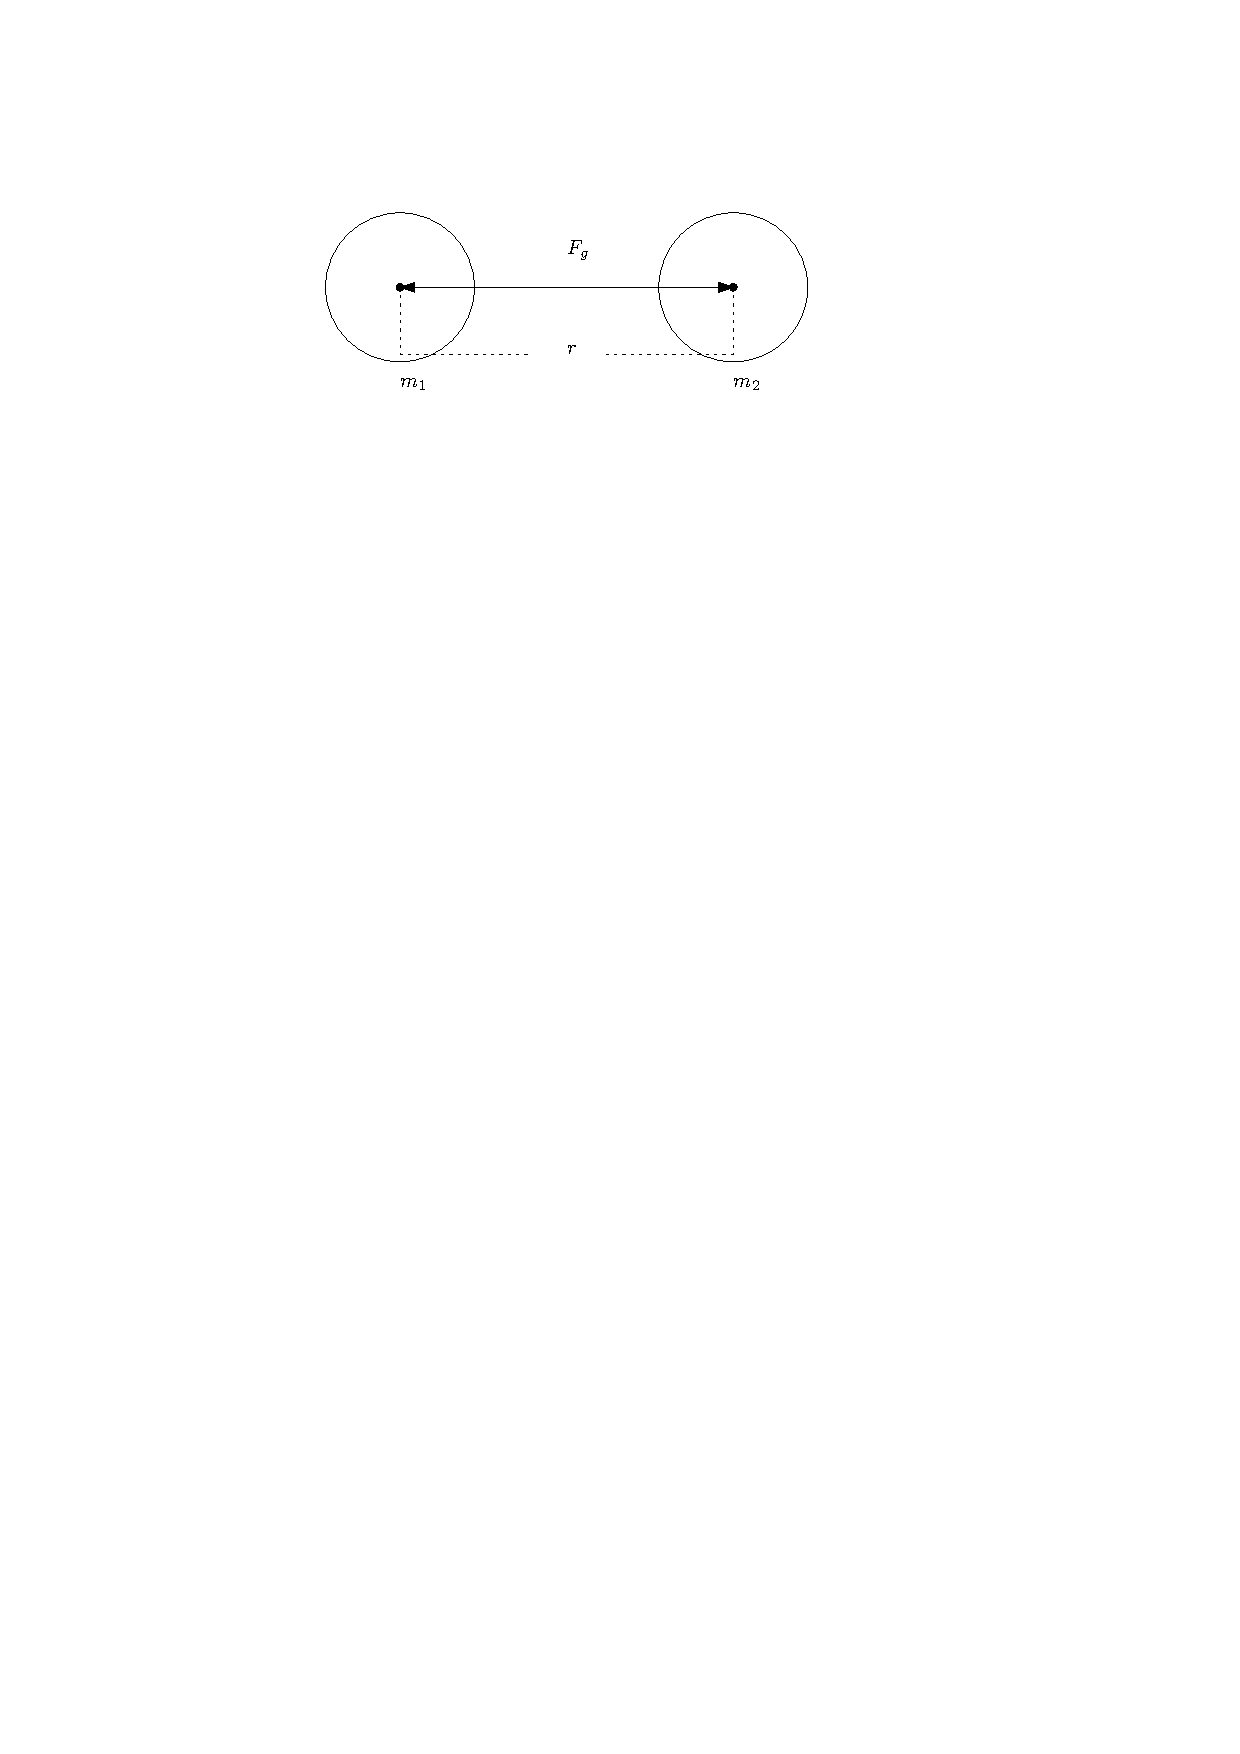
\includegraphics{massAttract}} \hfill
\vspace{1cm}
\parbox{10cm}{Newton discovered that the force of gravity between two objects is directly proportional to the product of their masses and inversely proportional to the square of the distance between them.} \hfill \mbox{\large $F \sim \frac{m_1 m_2}{r^2}$} \hfill
\vspace{1cm}

\hspace{3cm} \parbox{8cm}{The constant of proportionality is experimentally determined.  The first person to do this was Cavendish in 1798: \\ \\ $G = 6.674 \times 10^-{11}$ N$\cdot$m$^2$/cm$^2$} \hfill \mbox{\Large $F = G \frac{m_1 m_2}{r^2}$} \hfill
\vspace{1.5cm}

\hfill \parbox{10 cm}{When considering the gravitational attraction between two masses, all of the mass may be considered to be located at the center of mass of the object.} \hfill \mbox{} \\

\hfill 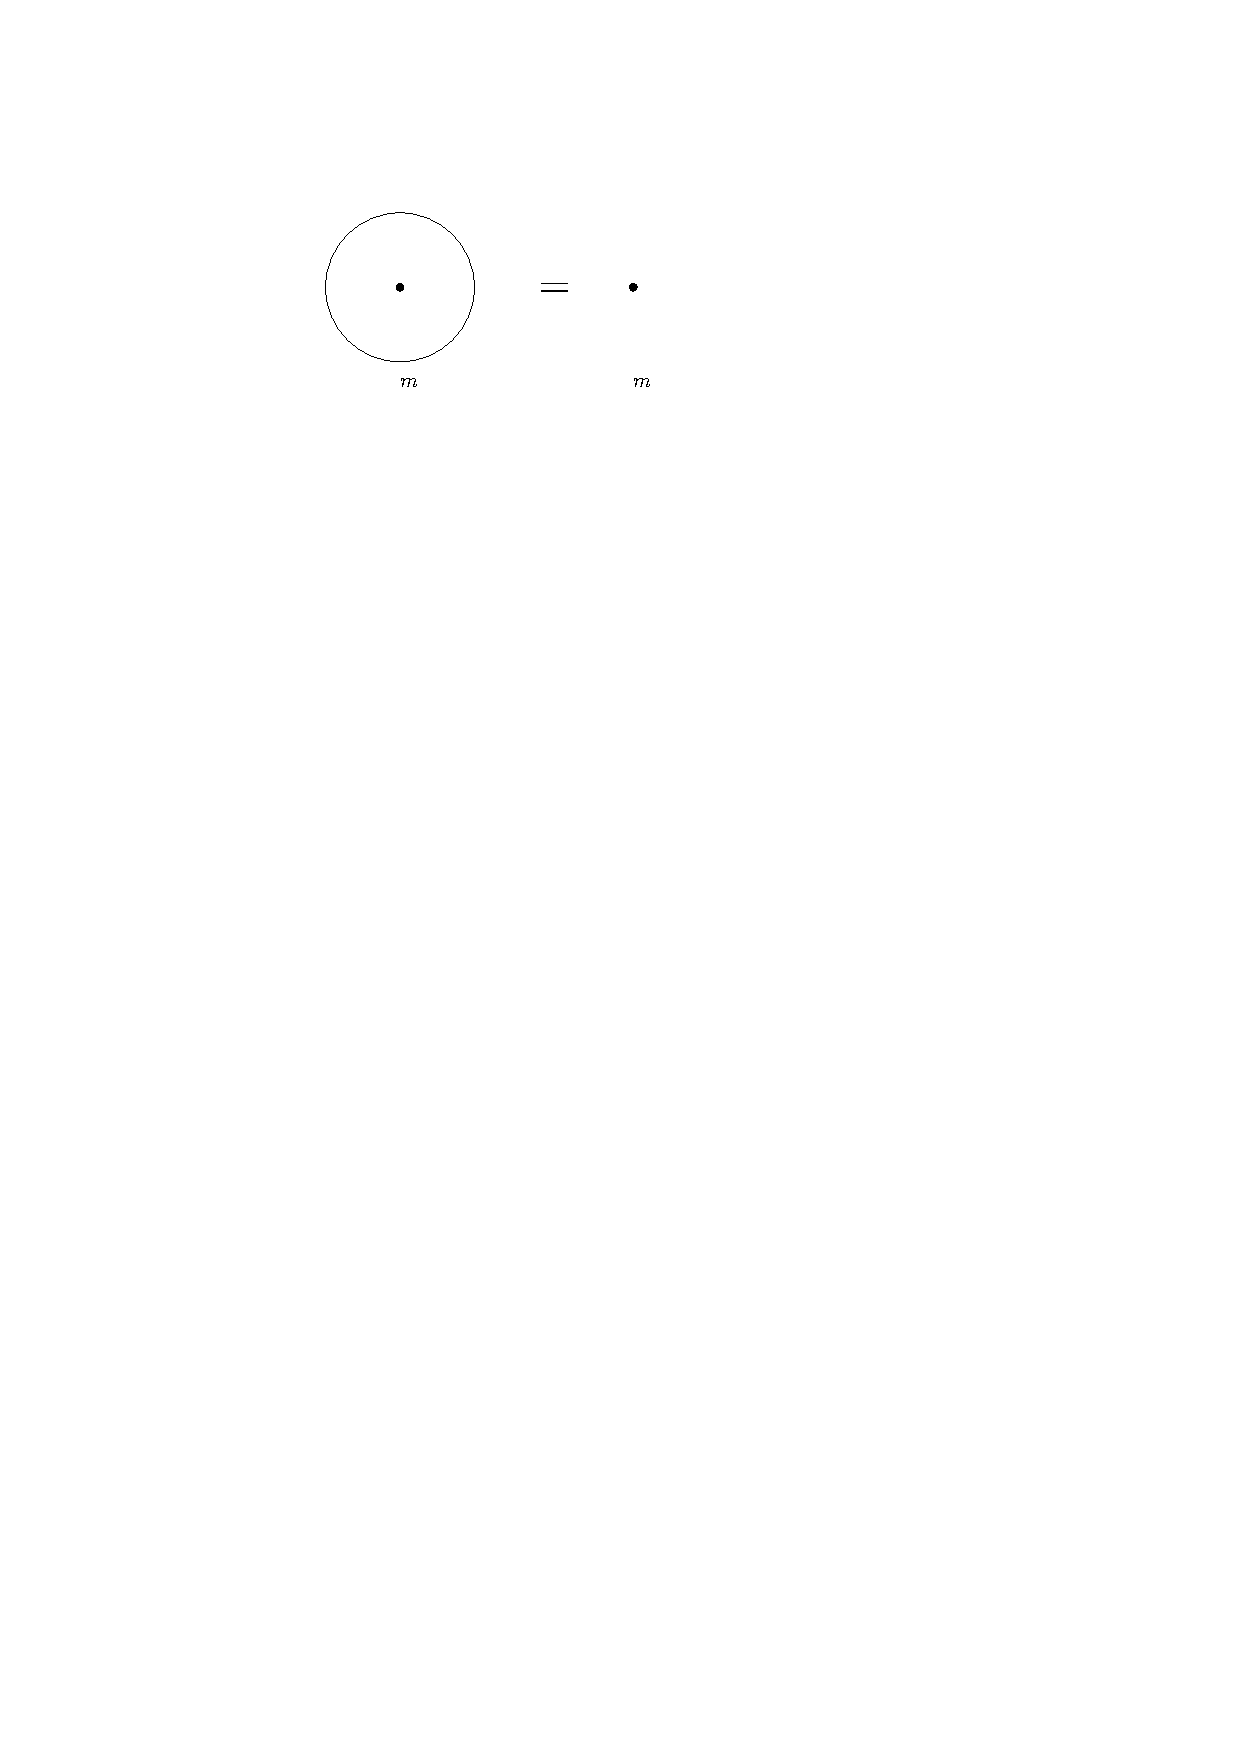
\includegraphics{cmEquiv} \hfill \mbox{} \\

\hfill \parbox{10cm}{\centering \emph{This is not an approximation.}} \hfill \mbox{} \\
\vspace{1cm}

\probDir{Important Constants} \\
mass of the sun = $1.9891 \times 10^{30}$kg \\
mass of the earth = $5.9722 \times 10^{24}$kg \\
mass of the moon = $7.3477 \times 10^{22}$kg\\
radius of earth = 6378 km \\
radius of moon = 1737 km \\
distance of earth to moon = 384400 km \\
distance of earth to sun = 149 597 870 km \\


\pagebreak

\probDir{Draw diagrams and show work on a separate sheet to answer the following problems.  Use Newton's Law of Universal Gravitation.}
\begin{enumerate}
\item What is the force of gravity on a 25 kg mass located on the surface of the earth?
\item Felix Baumgartner jumped out of a hot air balloon at an elevation of 39 km on Oct. 14, 2012.  Assuming he weighed 80 kg, what was the force of gravity on his body?
\item What was the acceleration due to gravity on Baumgartner's body?
\item What is the force of gravity on the Moon due to the Earth?
\item What is the force of gravity on the Earth due to the Moon?
\item What is the force of gravity on the Earth due to the Sun?
\item What is the acceleration due to gravity on the surface of the moon?
\item If an astronaut is exactly half way between the earth and the moon, calculate the net force on them.  Be sure to include direction.

\end{enumerate}

\end{document}